\include{mathbf}
\include{intercal}
\include{graphicx}
\section{Introduction}\raggedbottom

\subsection{Recommender System}
A recommender system is an information retrieval systems that aims to predict the rating of a user for a given item based on 
historical data.
This data can either be \textit{implicit} i.e. users in the system do not explicitly give ratings to items (e.g. clicks) or the data
can be \textit{explicit} i.e. users in the system provide explicit ratings for items (e.g. an amazon article rating).
\\
A distinction between between two types of recommender systems is made:
\begin{enumerate}
    \item Content-based recommender systems 
    \item Collaborative filtering recommender systems
\end{enumerate}

Content-based recommender systems exploit the attributes of items to make their recommendations.
This means that items are interpreted as similar if their attribute - values are similar. 
In content - based recommender systems the item - similarity is combined with the historical user - data to produce recommendations.
For this purpose a similarity - matrix \boldmath${A} \in \mathbf{R}^{nxn}$ (with $n$ being the number of items) is calculalated to find
similar items. The assumption that a content-based recommender system makes is that the ratings of one specific user strongly
correlate for similar items.

Collaborative filterting recommender systems expoits the similarity of users to make their recommendations. Only
implicit or explicit feedback provided by the users is used in this case. The goal is to find clusters of similar users i.e.
users whose rating-behaviour is similar. The assumption that a collaborative filtering recommender system makes is that
unspecified ratings can be imputed because the ratings of similar users for the same item strongly correlate.

\subsection{Matrix Factorization}
A matrix factorization decomposes a given matrix \boldmath${A} \in \mathbf{R}^{nxm}$ into the product \boldmath${B} \mathbf{C}^\top$ of two lower-dimensional matrices $B \in \mathbf{R}^{nxd}$ and $C \in \mathbf{R}^{mxd}$.
In the context of recommender systems the row of a matrix represents a user and the column of a matrix represents an item.
Each vector of the lower-dimensional matrix $B$ is the $d$-dimensional representation of a user. Likewise, each vector of the lower-dimensional matrix $C$
is the $d$-dimensional representation of an item.
The higher the dimension $d$, the more features of an item are found that a user can either like/dislike. 
Usually it holds that \boldmath$d << n,m$.
The goal of a matrix factorization is to approximate the original matrix $A$ by the product of the low-dimensional matrix \boldmath${B}$ and the
transposed low-dimensional matrix \boldmath$\mathbf{C}^\top$: \boldmath${A} \approx {B}\mathbf{C}^\top$.

\begin{figure}
    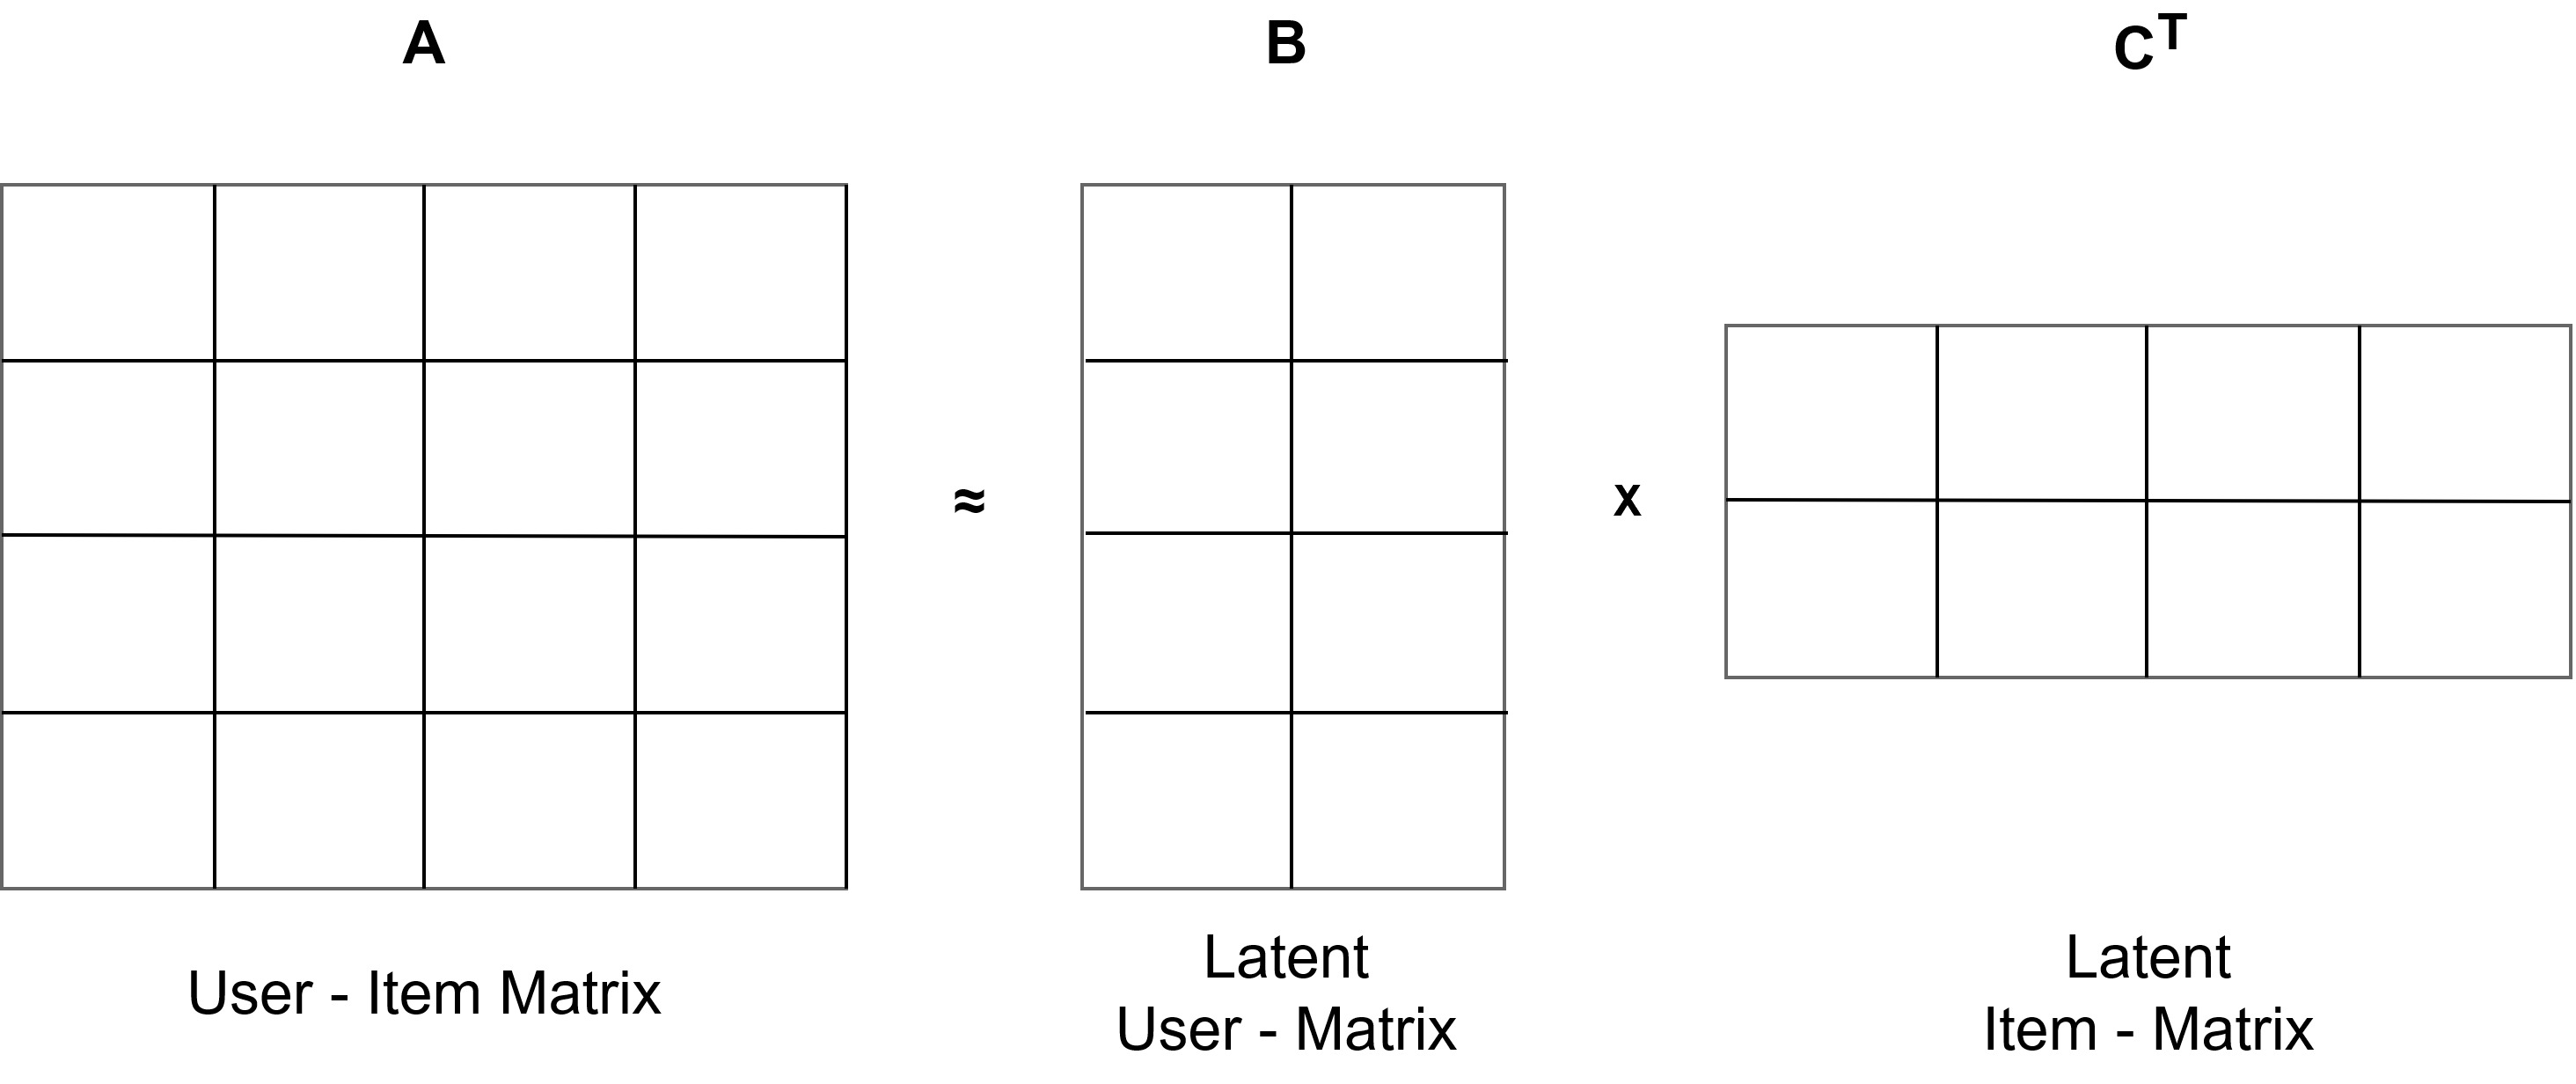
\includegraphics[width=\linewidth]{../images/matrix_factorization.jpg}
    \caption{}
    \label{Fig. 1.1: Matrix Factorization schema with embedding dimension d=2}
  \end{figure}
